\documentclass[11pt]{article}
\usepackage[margin=1in]{geometry}
\usepackage[T1]{fontenc}
\usepackage{lmodern}
\usepackage{booktabs}
\usepackage{amsmath}
\usepackage{graphicx}
\usepackage{xcolor}
\usepackage[hidelinks]{hyperref}
\usepackage{microtype}
\usepackage[round]{natbib}

\newcommand{\sumtok}{\texttt{<sum>}}

\title{Scope-Aligned Summary Tokens in a Hybrid-Attention Code Model:\\
A Controlled Study with a Negative Result}
\author{Anonymous}
\date{}

\begin{document}
\maketitle

\begin{abstract}
Summary (or ``gist'') tokens compress a span of context into a few positions,
so that later tokens can reach the span through them instead of through its
raw key--value entries. For source code, a natural place for such tokens is
the end of each syntactic scope (function, class, module run). We retrofit
this idea onto the sliding-window layers of Gemma~4~E2B with LoRA and compare
seven variants under matched token counts and, where it matters, matched
key--value (KV) memory: no summaries, fixed-interval chunks, scope-aligned
summaries, scope-local attention windows, call-graph edges between summaries,
and memory- and count-matched versions of the scope and chunk variants.
Across language-model loss, a long-range identifier loss, bug localization on
SWE-bench Lite and linear probes, no summary variant improves on the
no-summary baseline. A test-time ablation that hides every \sumtok{} token
changes long-range loss by at most $\pm 0.004$ nats, and the summaries receive
under 1\% of attention. Shrinking the local window from 512 to 128 tokens does
not change this: the model routes distant context through its full-attention
layers instead, whose attention to far tokens rises from 35\% to 57\%.
Linear probes do recover function properties from scope-aligned \sumtok{}
states far better than from fixed-chunk states (e.g.\ 0.92 vs.\ 0.71 on
\emph{returns a value}), but a mean of the function's own raw hidden states
does as well or better. So the probe advantage reflects \emph{where} the
summaries sit, not a learned compression. We conclude that in hybrid models
whose global layers see the full context, summary tokens added only to the
local layers are redundant. Removing that shortcut, by giving every layer the
same local mask, more than doubles long-range loss, and the summaries still do
not recover the lost context; keeping every function signature visible
recovers only a small part of it, and a SepLLM-style baseline that keeps
separator tokens does better than both, at a larger memory cost. All main
results hold across two training seeds.
\end{abstract}

\section{Introduction}

Long code contexts are expensive: KV memory grows linearly with length, and
most of a file is irrelevant to the next token. Context-compression methods
insert learned summary tokens that absorb a span and stand in for it
\citep{mu2023gist,chevalier2023autocompressor,ge2023icae,zhang2024beacon}.
Almost all of them place the tokens at fixed intervals. Code, however, has
explicit structure. A function is a natural unit of meaning, and a summary at
its end could serve later code that calls it.

We ask a narrow, controlled question: \emph{does placing summary tokens at
code-scope boundaries help, compared with placing the same number of tokens
at fixed intervals, when everything else is held fixed?} We study this in a
modern hybrid-attention model, Gemma~4~E2B. Its 35 layers repeat a pattern of
four sliding-window layers ($W=512$) and one full-attention layer. We change
only the attention masks of the sliding layers, so a raw token sees its last
$W$ raw tokens plus every earlier \sumtok{}, and each \sumtok{} sees the raw
tokens of its own segment. We then fine-tune with LoRA.

Our contributions are:
\begin{itemize}
\item A retrofit of scope-aligned summary tokens, with nesting and optional
  call-graph edges, onto the local layers of a pretrained hybrid model,
  without resizing its vocabulary or embeddings (\S\ref{sec:method}).
\item A controlled comparison with matched \sumtok{} counts and matched KV
  memory. Matching matters: the naive scope variant keeps 52\% more KV live
  than its fixed-chunk counterpart, because a long scope must stay in memory
  until its summary (\S\ref{sec:fair}).
\item Diagnostics that test whether the summaries are \emph{used}: test-time
  hiding, attention shares and loss by position in a scope. They show that
  the summaries are not used, and identify the full-attention layers as the
  reason (\S\ref{sec:results}).
\item Probe controls showing that the advantage of scope-aligned summaries on
  per-function probes is explained by their alignment, not by compression.
\item Tests with the global shortcut removed, two training seeds, a
  signature-keeping variant and a SepLLM-style baseline, placed on a
  memory--quality trade-off: at our budget, long-range quality follows how
  many raw tokens are kept, not the learned summaries (\S\ref{sec:discussion}).
\end{itemize}

\section{Related work}

\paragraph{Summary and gist tokens.}
Gist tokens \citep{mu2023gist}, AutoCompressors \citep{chevalier2023autocompressor},
ICAE \citep{ge2023icae} and Activation Beacon \citep{zhang2024beacon} compress
context into learned tokens, mostly at fixed intervals. Sentence-anchored gist
compression \citep{sentgist} anchors gists at sentence boundaries, but without
a matched uniform baseline. Gist-token sparse attention \citep{hssa} and adaptive
semantic trees \citep{admtree} organize summaries hierarchically. SepLLM \citep{chen2024sepllm} keeps separator tokens as
implicit summaries. Kwai Summary Attention \citep{kwaisummary} builds a hybrid stack of summary and
full-attention layers, with fixed chunks, trained from scratch or with
continued pretraining on far more tokens than we use.

\paragraph{Compression for code.}
CodeComp \citep{codecomp} compresses the KV cache using a code property graph,
without training. \citet{skipcompressor} report that compressors hurt
repository-level issue fixing. We are not aware of prior work that places
\emph{learned} summaries at code-scope boundaries, nests them along the scope
tree, compares boundary and uniform placement at matched count and memory, or
links summaries along call edges.

\paragraph{Attention sinks.}
\citet{xiao2023sinks} show that models park attention on a few tokens, such as
the first token. Our diagnostics test whether \sumtok{} attention reflects
information transfer or sink behaviour.

\section{Method}\label{sec:method}

\begin{figure}[t]
\centering
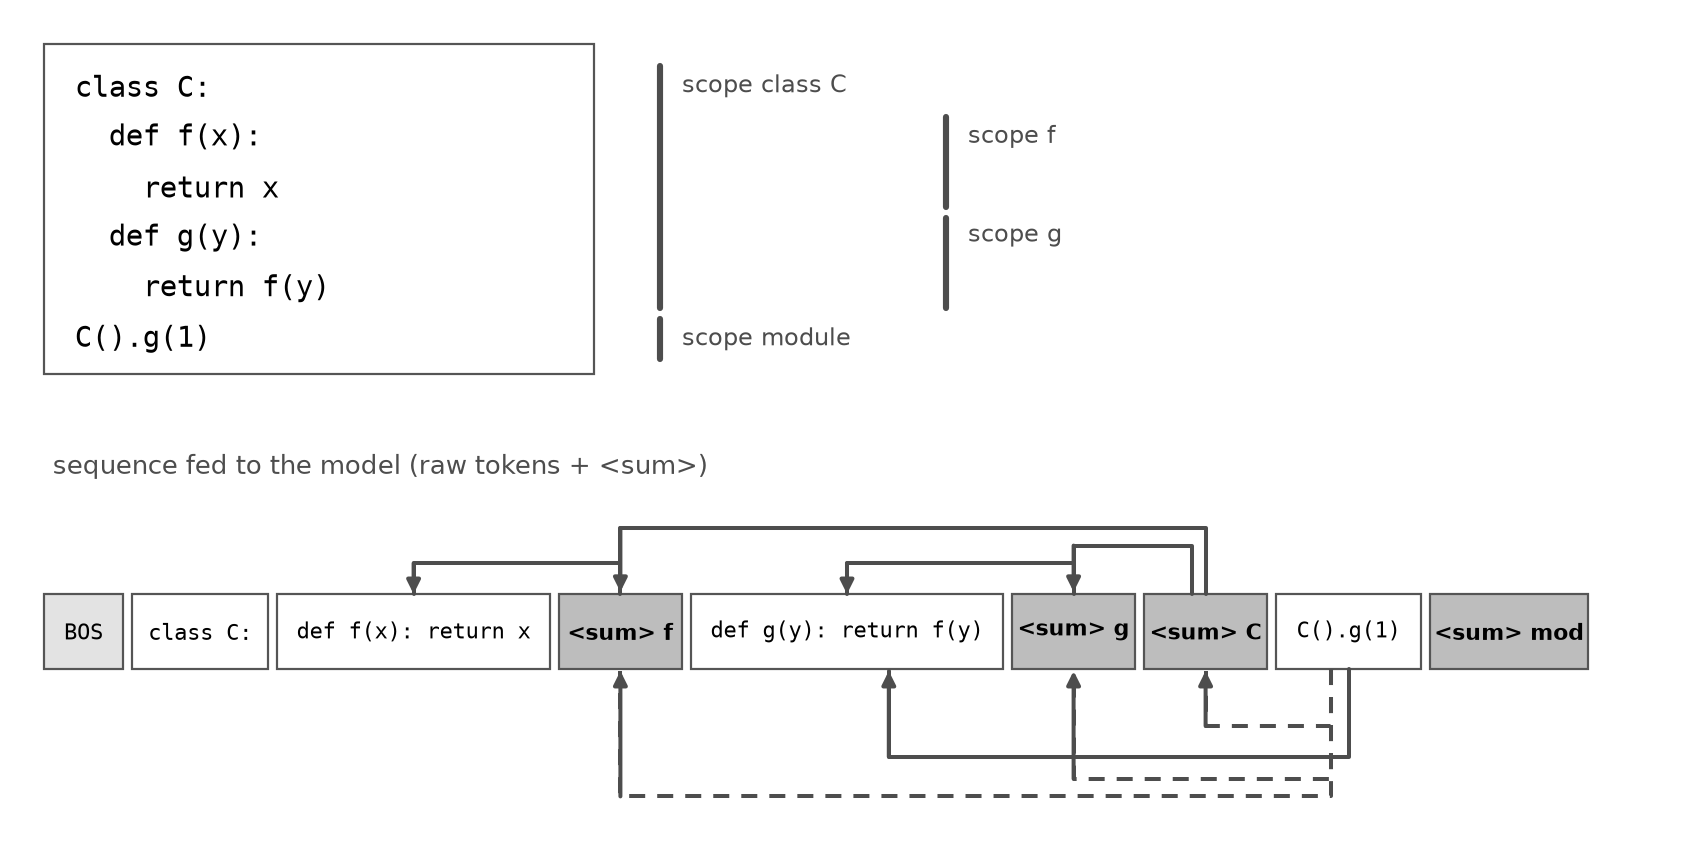
\includegraphics[width=0.92\textwidth]{figures/fig_insertion.png}
\caption{Inserting summary tokens. A scope tracker splits the code into
nested scopes, and a \sumtok{} token is inserted after the last raw token of
each scope. Above the sequence: a \sumtok{} query attends to its scope's raw
tokens and to the \sumtok{}s of nested scopes. Below: a raw query in a
sliding layer attends to the last $W$ raw tokens (solid) and to every earlier
\sumtok{} (dashed). Variant F splits a long scope into parts of at most $W$
tokens, each with its own \sumtok{}; B and G place the same number of
\sumtok{}s every $K$ raw tokens instead.}
\label{fig:insert}
\end{figure}


\paragraph{Segments.}
A logical-line lexer and an indentation stack split a Python window into
\emph{scopes}: functions and classes (with their decorators), plus
\emph{module runs} between top-level definitions. Each scope's raw tokens are
the tokens directly inside it. Tokens of nested scopes belong to the nested
scope, and the scope's header (e.g.\ the \texttt{def} line) is marked. One
\sumtok{} is inserted right after the last raw token of each segment. Each
variant defines segments differently (Table~\ref{tab:variants}).
Figure~\ref{fig:insert} shows this on a small example.

\paragraph{Masks.}
Global (full-attention) layers stay causal. In the sliding layers, for
variants B, C, F and G, a raw query sees BOS, the last $W$ raw tokens (counted
in raw tokens) and every earlier \sumtok{}. A \sumtok{} query sees BOS, the raw
tokens of its own segment and the \sumtok{}s of its direct children. D and E
replace the $W$-token window with the query's own scope, the headers of
enclosing scopes and the last $w=64$ tokens. E also lets a \sumtok{} attend to
the \sumtok{}s of functions it calls (call edges found by regular expressions).

Formally, let $\kappa(j)\in\{\textsc{bos},\textsc{raw},\textsc{sum}\}$ be the
kind of position $j$, $r(j)$ its index among raw tokens, $s(j)$ its segment,
and $\pi(g)$ the parent segment of $g$. In a sliding layer of variants B, C, F
and G, a raw query $q$ may attend to key $k\le q$ when
\begin{equation}
\begin{aligned}
&\kappa(k)=\textsc{bos} \;\lor\; \kappa(k)=\textsc{sum}\\
&\;\lor\; \bigl(\kappa(k)=\textsc{raw} \land r(q)-r(k)<W\bigr),
\end{aligned}
\label{eq:rawmask}
\end{equation}
and a \sumtok{} query $q$ may attend to $k\le q$ when
\begin{equation}
\begin{aligned}
&\kappa(k)=\textsc{bos} \;\lor\; \bigl(\kappa(k)=\textsc{raw}\land s(k)=s(q)\bigr)\\
&\;\lor\; \bigl(\kappa(k)=\textsc{sum}\land \pi(s(k))=s(q)\bigr).
\end{aligned}
\label{eq:summask}
\end{equation}
Full-attention layers use the plain causal mask ($k\le q$) unless
\texttt{restrict\_full} is set, in which case they use
(\ref{eq:rawmask})--(\ref{eq:summask}) as well. Every position also attends to
itself, and padding is never attended.
Figure~\ref{fig:mask} shows the sliding mask for the example of
Figure~\ref{fig:insert}, and Figure~\ref{fig:layers} shows where these masks
sit in the model.

\begin{figure}[t]
\centering
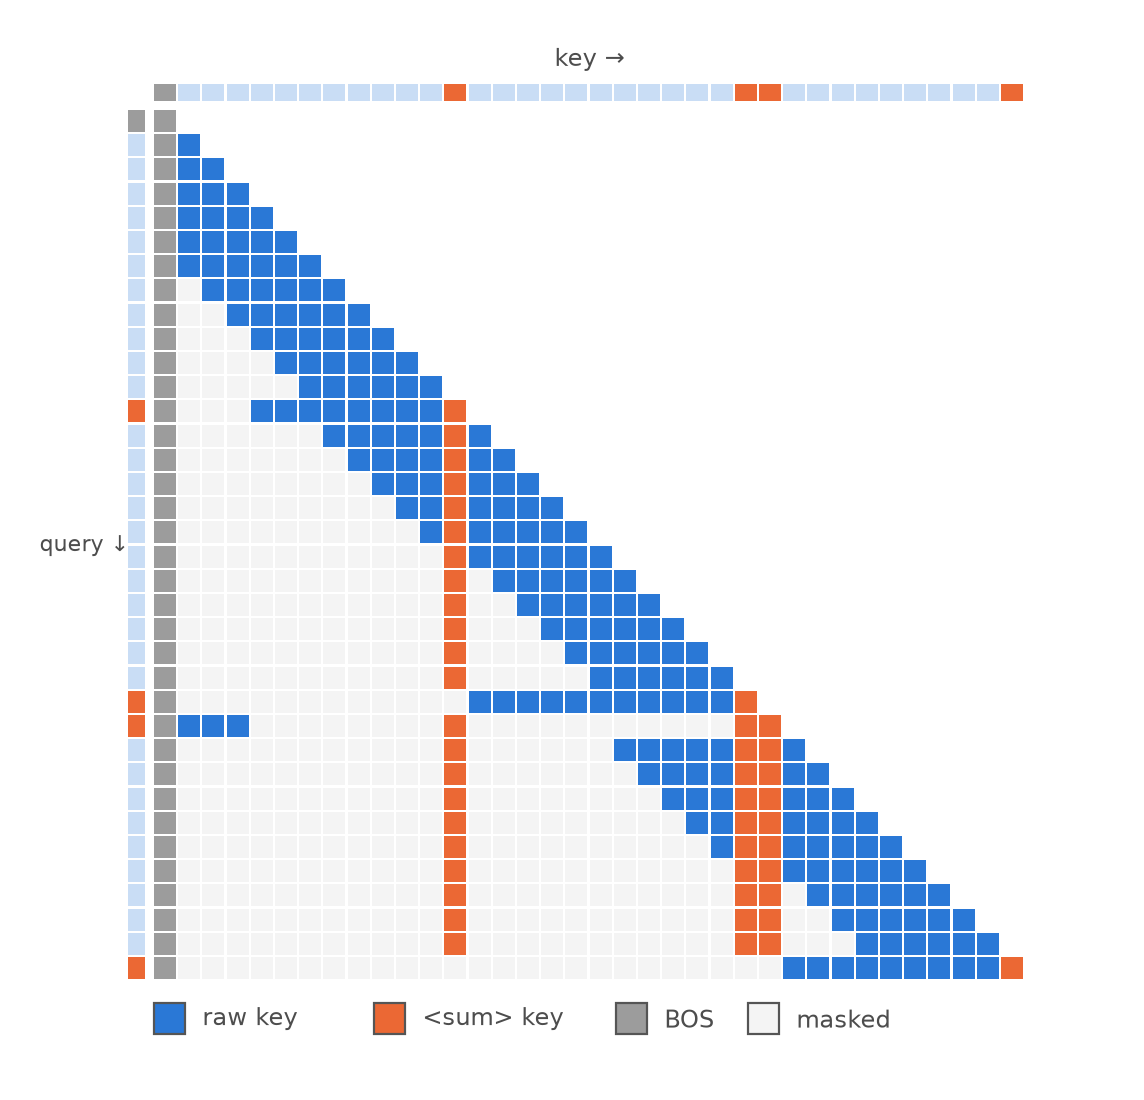
\includegraphics[width=0.48\textwidth]{figures/fig_mask.png}
\caption{The sliding-layer mask our code builds for the example of
Figure~\ref{fig:insert} (variant C, $W=6$; row = query, column = key). Raw
rows see a band of the last $W$ raw tokens plus every earlier \sumtok{};
\sumtok{} rows see their own scope's raw tokens and the \sumtok{} of nested
scopes.}
\label{fig:mask}
\end{figure}

\begin{figure}[t]
\centering
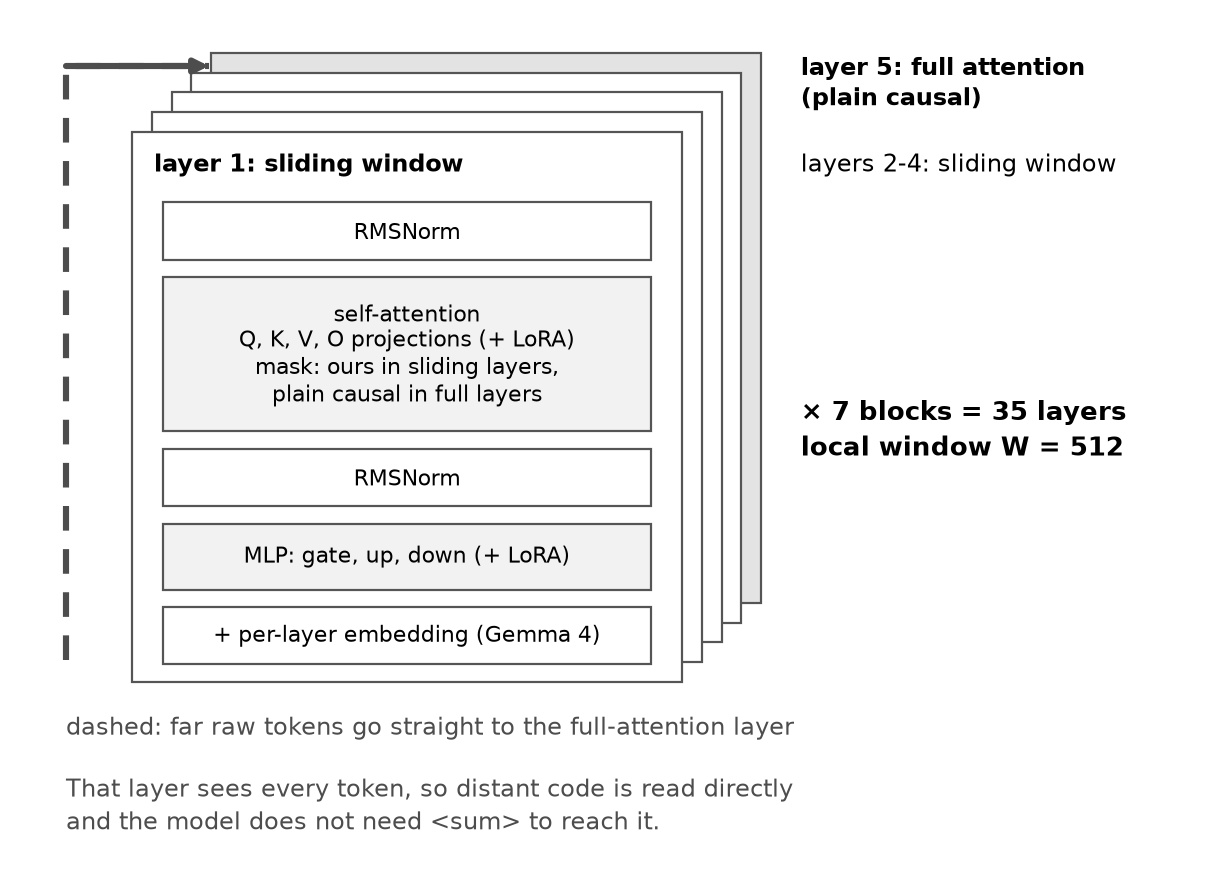
\includegraphics[width=0.62\textwidth]{figures/fig_layers.png}
\caption{Where the masks apply. Gemma~4~E2B stacks 7 blocks of five layers;
the front layer shows what each layer contains. Our masks replace only the
attention mask of the four sliding-window layers. The fifth layer uses full
attention and still sees every token, so far code can reach it directly
(dashed path).}
\label{fig:layers}
\end{figure}

\paragraph{Retrofit.}
Gemma~4 reserves thousands of unused tokens, so we reuse \texttt{<unused0>} as
\sumtok{}. Its input embedding is a trainable vector initialised to the mean
embedding row, and its per-layer-embedding row is reset to the mean. We pass
per-layer-type masks to the decoder as a dictionary, so the library's own
sliding-window mask is replaced only in the sliding layers.

\begin{table}[t]
\centering\small
\begin{tabular}{@{}lll@{}}
\toprule
& Segments & Sliding-layer raw query sees \\
\midrule
A & none & last $W$ positions (model default) \\
B & fixed chunks, $K=223$ (count-matched to C) & last $W$ raw + all earlier \sumtok{} \\
C & scopes & last $W$ raw + all earlier \sumtok{} \\
D & scopes & own scope + enclosing headers + last 64 + all \sumtok{} \\
E & scopes, + callee edges between \sumtok{} & as D \\
F & scopes, long scopes split into parts $\le W$ & as C \\
G & fixed chunks, $K=180$ (count-matched to F) & as B \\
S & none (SepLLM-style baseline) & last $W$ raw + every earlier separator \\
\bottomrule
\end{tabular}
\caption{Variants. All use identical windows, data order and hyper-parameters.
Two options change the masks: \texttt{restrict\_full} gives the
full-attention layers the same mask as the sliding layers (otherwise they
see every earlier token), and \texttt{keep\_signatures} lets raw queries also
see every earlier \texttt{def}/\texttt{class} line. Separators (S) are
whitespace tokens and \texttt{.}~\texttt{,}~\texttt{?}~\texttt{!}~\texttt{;}~\texttt{:}.}
\label{tab:variants}
\end{table}

\subsection{Fair comparison}\label{sec:fair}

B fixes the \emph{count} of summary tokens. Its $K$ is chosen so that the
total number of fixed-chunk \sumtok{}s over the training set matches C's
(7.09 per window for both). Count matching is not enough,
because the two variants differ in KV memory. In C, the raw tokens of a
2{,}000-token class body must stay in the cache until the class's \sumtok{}
has attended to them. The measured mean live KV is 672 entries for C and 441
for B, and the peak is 1{,}193 vs.\ 521. F removes this advantage. It cuts any
scope whose span exceeds $W$ into consecutive \emph{parts} at logical-line
starts. Each part gets a \sumtok{} and becomes a child of the scope, and the
scope's header goes into its first part. With $W=512$ on the training
windows, F's live KV matches B's (mean 289 vs.\ 288, peak 517 vs.\ 516).%
\footnote{The F evaluation in Table~\ref{tab:main} was run before the header
fix and reports peak 776; loss and probes are unaffected by where headers are
kept in memory.}
G re-fits $K$ so that fixed chunks match F's count (57{,}820 vs.\ 59{,}900
\sumtok{}s over the training set). Figure~\ref{fig:kv} shows the memory of
all variants on the evaluation windows.

\begin{figure}[t]
\centering
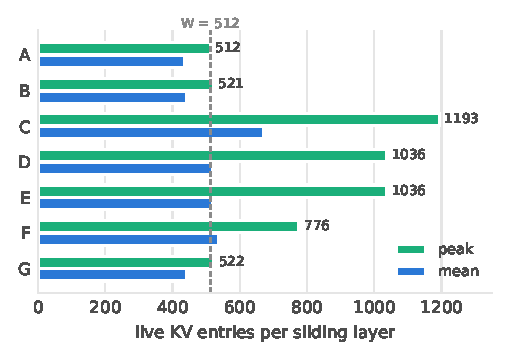
\includegraphics[width=0.55\textwidth]{figures/kv.pdf}
\caption{Live KV entries per sliding layer on the evaluation windows (mean
and peak over positions). C, D and E keep long scopes in memory until their
\sumtok{}; B and G stay at about $W$. F was measured before the header fix
(peak 776); after it, F's peak matches B's on the training windows.}
\label{fig:kv}
\end{figure}

\section{Experimental setup}

\paragraph{Data.}
Python files from The Stack \citep{kocetkov2022stack} (\texttt{the-stack-smol-xl}).
We exclude the four evaluation repositories (fastapi, requests, rich, httpx)
by name, path and signature, and the twelve SWE-bench Lite repositories by
exact name. Files are cut into windows of at most 1{,}791 raw tokens at
top-level boundaries, leaving room for summaries in a 2{,}048-token
sequence. This gives 6{,}967 training windows (10M tokens).

\paragraph{Training.}
LoRA \citep{hu2021lora} with rank 16 and $\alpha=32$ on all attention and MLP
projections of the text decoder, with learning rate $2\times10^{-4}$
($10^{-3}$ for the \sumtok{} embedding). Effective batch 16, 130 steps (about
3M tokens), 13 warm-up steps, float16 on one T4 GPU, about 2.7 hours per
variant, two seeds (1234 and 2) for every variant in Table~\ref{tab:seeds}. Table~\ref{tab:setup} lists the full setup, and
Figure~\ref{fig:train} shows the training loss of the main runs.

\begin{table}[t]
\centering\small
\begin{tabular}{@{}ll@{}}
\toprule
Setting & Value \\
\midrule
Base model & Gemma~4~E2B (28 sliding + 7 full) \\
Sliding window $W$ & 512 (128 in the stress test) \\
Adapter & LoRA, $r=16$, $\alpha=32$, dropout 0.05 \\
LoRA targets & q, k, v, o, gate, up, down \\
\sumtok{} token & reused \texttt{<unused0>}, trainable embedding \\
Learning rate & $2\times10^{-4}$ (LoRA), $10^{-3}$ (\sumtok{}) \\
Schedule & 13 warm-up steps, then decay to 0 \\
Batch & 1 window $\times$ 16 accumulation steps \\
Steps / tokens & 130 / about 3M raw tokens \\
Sequence length & 2{,}048 (at most 1{,}791 raw + \sumtok{}) \\
Precision / hardware & float16 / one NVIDIA T4 (Kaggle) \\
Seeds & 1234; also 2 (Table~\ref{tab:seeds}) \\
\bottomrule
\end{tabular}
\caption{Training setup, identical for every variant.}
\label{tab:setup}
\end{table}

\begin{figure}[t]
\centering
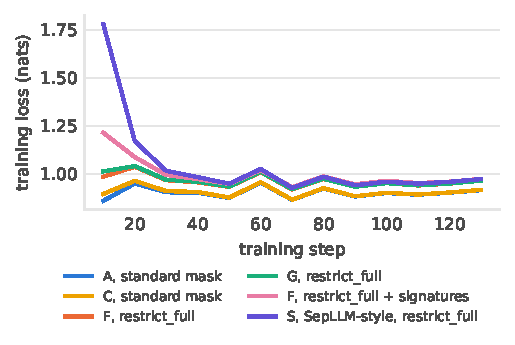
\includegraphics[width=0.55\textwidth]{figures/train_curves.pdf}
\caption{Training loss of the main runs (logged every 10 steps). Runs with the
same mask track each other because all variants see the same windows in the
same order; \texttt{restrict\_full} raises the loss throughout training.}
\label{fig:train}
\end{figure}

\paragraph{Evaluation.}
(i) Heldout LM loss on 99{,}657 tokens. (ii) Long-range identifier loss on 206
windows from the four held-out repositories: the loss on the 2{,}192
identifier tokens whose definition lies more than 512 raw tokens earlier
\emph{and} in a different scope. The target set is identical for all variants.
(iii) Bug localization on 19 SWE-bench Lite tasks \citep{jimenez2023swebench}:
every function in the patched files is ranked by the log-likelihood of its
name after the file and the issue text. (iv) Logistic-regression probes on
the last-layer \sumtok{} state of each function (1{,}191 train, 347 test
functions, split by file) for \emph{returns a value}, \emph{number of
arguments} (4 buckets) and \emph{name reused later}. For chunk variants the
probe uses the chunk containing the function's last token. Controls: the mean
of the function's raw hidden states (\emph{raw-mean}), and the subset of
functions that straddle a chunk boundary. (v) Diagnostics: loss with raw
queries blocked from all \sumtok{} keys (\emph{hide}), attention mass on
\sumtok{}, BOS and far raw tokens (eager attention, 16 windows), and loss by
offset from scope start.

\section{Results}\label{sec:results}

\begin{figure}[t]
\centering
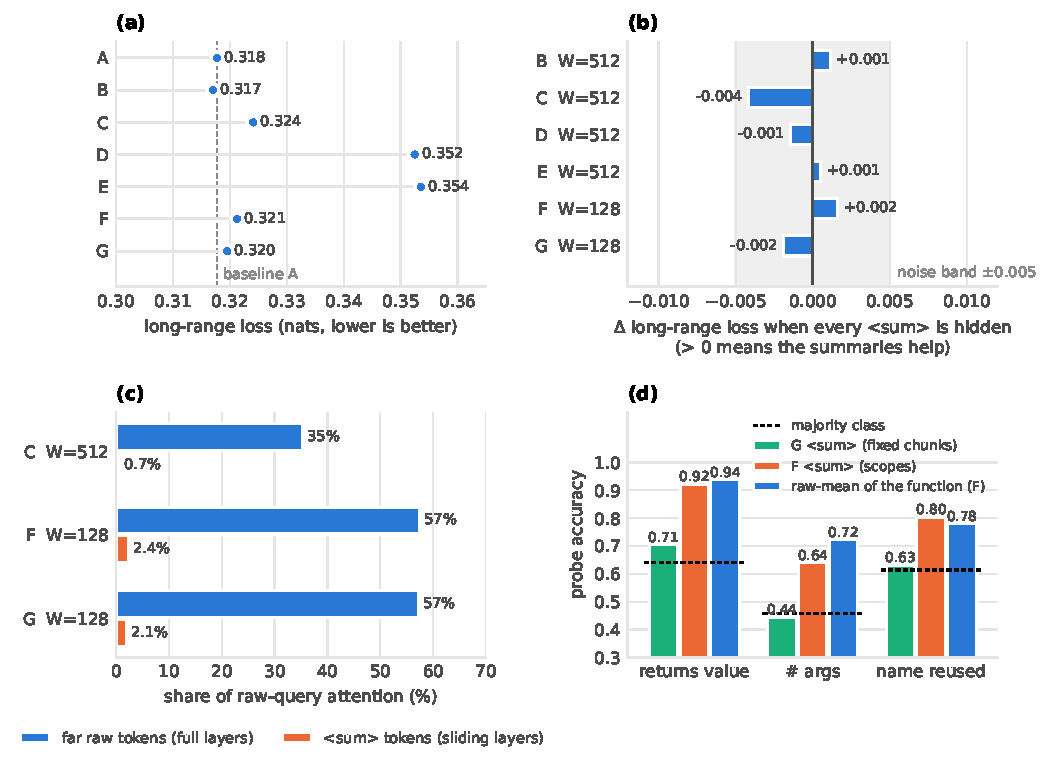
\includegraphics[width=\textwidth]{figures/results.pdf}
\caption{Summary of the results. (a) Long-range loss: no variant beats the
baseline A. (b) Hiding every \sumtok{} at test time changes long-range loss
by less than the noise band, in both directions. (c) The full-attention
layers carry distant context (35\% of their attention at $W=512$, 57\% at
$W=128$), while the \sumtok{} tokens get a few percent. (d) Scope-aligned
\sumtok{} states (F) encode function properties far better than
fixed-chunk ones (G), but no better than the mean of the function's raw
hidden states.}
\label{fig:results}
\end{figure}

\begin{table}[t]
\centering\small
\begin{tabular}{@{}lccccc@{}}
\toprule
& Heldout & All-token & Long-range & Live KV & Loc.\ top-1 / top-5 \\
& loss & loss (eval) & loss & mean / peak & (of 19) \\
\midrule
A baseline & \textbf{1.989} & \textbf{0.722} & 0.318 & 437 / 512 & 4 / 10 \\
B chunks ($K$=223) & 1.992 & 0.724 & \textbf{0.317} & 441 / 521 & 3 / 9 \\
C scopes & 1.991 & 0.724 & 0.324 & 672 / 1193 & 3 / 11 \\
D scope windows & 2.020 & 0.750 & 0.352 & 519 / 1036 & 4 / 9 \\
E + call edges & 2.021 & 0.749 & 0.354 & 519 / 1036 & 4 / 9 \\
F scopes, parts $\le W$ & 1.991 & 0.724 & 0.321 & 536 / 776 & 3 / 11 \\
G chunks ($K$=180) & 1.993 & 0.726 & 0.320 & 442 / 522 & 3 / 9 \\
\bottomrule
\end{tabular}
\caption{Main results at $W=512$. Lower loss is better. Differences below
about 0.01 nats are within run-to-run noise (seed 1; Table~\ref{tab:seeds} adds
seed 2).}
\label{tab:main}
\end{table}

\paragraph{No variant beats the baseline.}
Table~\ref{tab:main} and Figure~\ref{fig:results}a show heldout and long-range losses within 0.004 nats of
each other for A, B, C, F and G. D and E are 0.03 nats worse: their raw
queries lose the most recent 512 tokens outside their own scope, and the
summaries do not make up for it. Bug localization does not separate the
variants on 19 tasks. A second seed (Table~\ref{tab:seeds}) moves A's
long-range loss by 0.007 (0.318 to 0.325), more than the gaps between A, F
and G (0.320--0.322 in seed 2), so with the standard mask there is no
measurable difference between them.

\begin{table}[t]
\centering\small
\begin{tabular}{@{}llccccc@{}}
\toprule
& & \multicolumn{3}{c}{Long-range loss} & \multicolumn{2}{c}{$\Delta$ when \sumtok{} hidden} \\
\cmidrule(lr){3-5}\cmidrule(l){6-7}
Mask & Variant & seed 1 & seed 2 & mean & seed 1 & seed 2 \\
\midrule
standard & A & 0.318 & 0.325 & 0.321 & -- & -- \\
standard & F & 0.321 & 0.321 & 0.321 & $-0.003$ & $-0.0003$ \\
standard & G & 0.320 & 0.322 & 0.321 & $-0.0001$ & $-0.004$ \\
\texttt{restrict\_full} & F & 0.735 & 0.720 & 0.728 & $-0.008$ & $-0.014$ \\
\texttt{restrict\_full} & G & 0.694 & 0.713 & 0.704 & $-0.004$ & $-0.001$ \\
\texttt{restrict\_full} & F + signatures & 0.691 & 0.694 & 0.693 & $-0.001$ & $-0.002$ \\
\texttt{restrict\_full} & S (SepLLM-style) & 0.632 & 0.630 & 0.631 & -- & -- \\
\bottomrule
\end{tabular}
\caption{Two training seeds (seed 2 changes the LoRA initialisation and the
data order). $\Delta$ is the change in long-range loss when every \sumtok{}
is hidden at test time; it stays at or below zero in all 13 diagnosed runs.
Seed 1 of F (standard mask) was trained before long scopes moved their
header into the first part and diagnosed after, so its segments differ
slightly from training. S has no \sumtok{} to hide.}
\label{tab:seeds}
\end{table}

\begin{table}[t]
\centering\small
\begin{tabular}{@{}llcccc@{}}
\toprule
& & \sumtok{} attention & Far-raw attention & \multicolumn{2}{c}{$\Delta$ loss when hidden} \\
$W$ & Var. & sliding / full & full layers & long-range & all \\
\midrule
512 & B & 1.0\% / 0.6\% & 35\% & $+0.001$ & $-0.001$ \\
512 & C & 0.7\% / 0.3\% & 35\% & $-0.004$ & $-0.001$ \\
512 & D & 0.8\% / 0.3\% & 33\% & $-0.001$ & $-0.001$ \\
512 & E & 0.7\% / 0.4\% & 34\% & $+0.001$ & $-0.000$ \\
128 & F & 2.4\% / 0.6\% & 57\% & $+0.002$ & $-0.000$ \\
128 & G ($K$=90) & 2.1\% / 0.9\% & 57\% & $-0.002$ & $-0.000$ \\
\bottomrule
\end{tabular}
\caption{Are the summaries used? $\Delta$ is the change in loss when every raw
query is blocked from every \sumtok{} at test time. A positive value means the
summaries help. Far-raw: attention from raw queries to raw keys more than $W$
tokens back, which only the full-attention layers can see.}
\label{tab:diag}
\end{table}

\begin{figure}[t]
\centering
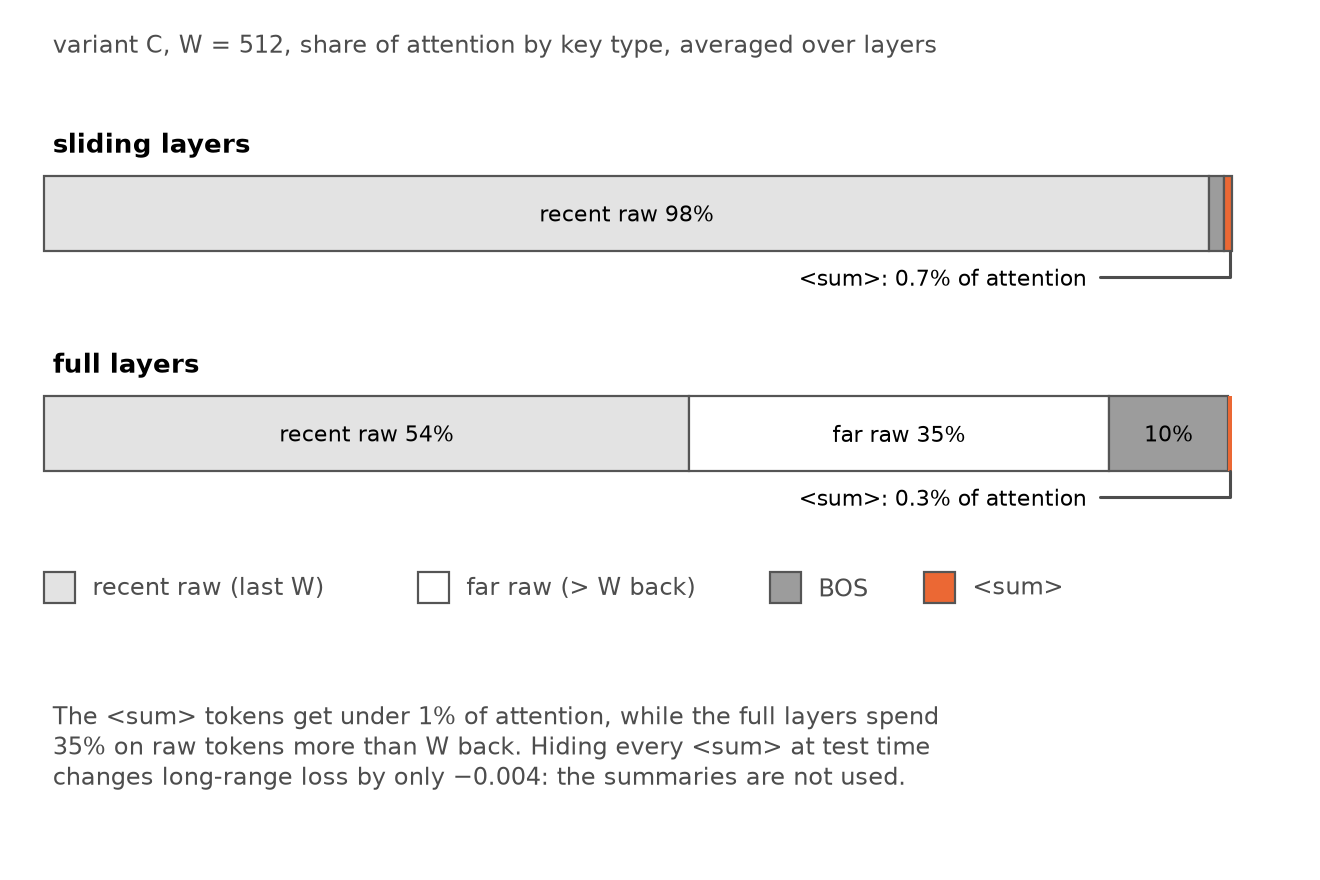
\includegraphics[width=0.62\textwidth]{figures/fig_attention.png}
\caption{Where a raw query's attention goes, measured on variant C at
$W=512$. \sumtok{} keys receive 0.7\% of attention in the sliding layers and
0.3\% in the full-attention layers, while the full layers spend 35\% on raw
tokens more than $W$ back.}
\label{fig:attn}
\end{figure}

\paragraph{The summaries are not used.}
Hiding all \sumtok{} keys at test time changes long-range loss by $-0.004$ to
$+0.001$ nats at $W=512$ (Table~\ref{tab:diag}, Figure~\ref{fig:results}b). In C, hiding them slightly
\emph{improves} the loss. The summaries receive under 1\% of attention (Figure~\ref{fig:attn}), about
a tenth of what BOS receives in the full-attention layers (10\%). Loss by
offset from the start of a scope, where a summary of the preceding code
should help most, is the same for A, B and C (0.977, 0.979 and 0.982 nats on
the first 16 tokens; Table~\ref{tab:offset}).

\begin{table}[t]
\centering\small
\begin{tabular}{@{}llcccc@{}}
\toprule
& & \multicolumn{4}{c}{offset from scope start (tokens)} \\
\cmidrule(l){3-6}
Mask & Variant & 0--15 & 16--63 & 64--255 & 256+ \\
\midrule
standard & A & 0.977 & 0.798 & 0.688 & 0.645 \\
standard & B & 0.979 & 0.800 & 0.690 & 0.647 \\
standard & C & 0.982 & 0.800 & 0.689 & 0.647 \\
\texttt{restrict\_full} & F & 1.027 & 0.838 & 0.718 & 0.684 \\
\texttt{restrict\_full} & G & 1.021 & 0.835 & 0.719 & 0.683 \\
\texttt{restrict\_full} + signatures & F & 1.023 & 0.852 & 0.739 & 0.704 \\
\texttt{restrict\_full} & S (SepLLM-style) & 1.025 & 0.844 & 0.728 & 0.697 \\
\bottomrule
\end{tabular}
\caption{All-token loss by position within the enclosing scope, $W=512$.
Summaries give no gain at scope starts, where earlier code should matter most.}
\label{tab:offset}
\end{table}

\begin{figure}[t]
\centering
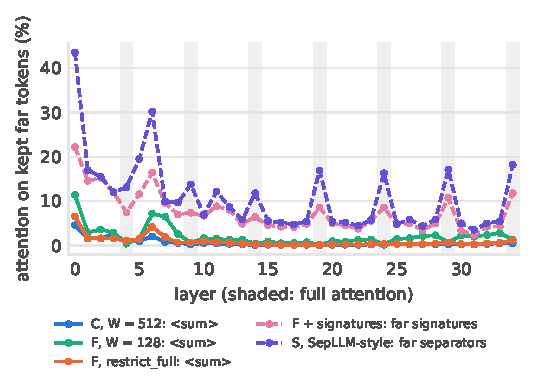
\includegraphics[width=0.55\textwidth]{figures/layer_attention.pdf}
\caption{Per layer (shaded: full attention), the share of raw-query
attention on the tokens each variant keeps beyond the window: \sumtok{} keys
(C, F) or kept raw tokens more than $W$ back (signatures, separators). The
model attends to kept raw tokens heavily (separators up to 43\%, signatures
up to 22\%) but to the summaries mostly below 2\%, even when they are the
only route past $W$ (\texttt{restrict\_full}).}
\label{fig:layerattn}
\end{figure}

Per layer (Figure~\ref{fig:layerattn}), the little attention the summaries
receive is concentrated in the first layers (up to 11\% in layer 0 at
$W=128$) and stays below about 2\% in the later layers, where the model
forms its predictions; closing the shortcut does not move it there. Raw
tokens kept beyond the window are used very differently: signatures receive
5--22\% and separators 10--43\% of attention in many layers.

\paragraph{Why: the global layers already see everything.}
In the full-attention layers, 35\% of the attention of raw queries goes to raw
tokens more than 512 positions back. Distant code is therefore available
without the summaries. To test whether a narrower local window would force
the model to use them, we retrained F and G with $W=128$ (G with $K=90$ to
match F's count). The loss cost is small (heldout 2.004 and 2.008 vs.\
1.991). Attention to \sumtok{} rises to 2.4\%, but hiding the summaries still
changes long-range loss by only $\pm0.002$. The model instead shifts distant
context to the full-attention layers, whose far-raw share rises (Figure~\ref{fig:results}c) from 35\% to
57\%.

\begin{table}[t]
\centering\small
\begin{tabular}{@{}lcccccc|cc@{}}
\toprule
& \multicolumn{6}{c|}{\sumtok{} state} & \multicolumn{2}{c}{raw-mean} \\
Task (majority) & B & C & D & E & F & G & F & G \\
\midrule
returns value (0.640) & 0.709 & 0.905 & 0.885 & \textbf{0.939} & 0.922 & 0.706 & \textbf{0.939} & 0.934 \\
\# args (0.458) & 0.401 & 0.614 & 0.611 & 0.617 & 0.640 & 0.444 & \textbf{0.723} & 0.709 \\
name reused (0.614) & 0.602 & 0.790 & 0.795 & \textbf{0.813} & 0.804 & 0.631 & 0.781 & 0.767 \\
\bottomrule
\end{tabular}
\caption{Probe accuracy on held-out functions. Scope-aligned \sumtok{} states
(C--F) carry far more information about their function than fixed-chunk
states (B, G), but no more than the mean of the function's raw hidden states.
On the 181 functions that straddle a chunk boundary, \emph{returns a value}
is 0.906 for F, 0.680 for G and 0.928 for raw-mean.}
\label{tab:probe}
\end{table}

\paragraph{What the summary states contain.}
Probes on scope-aligned \sumtok{} states predict function properties well
above the majority class, and well above fixed-chunk states
(Table~\ref{tab:probe}, Figure~\ref{fig:results}d): \emph{returns a value} reaches 0.92 for F and 0.71
for G. The gap is largest for functions that straddle a chunk boundary, where
no single chunk summary covers the function (0.906 vs.\ 0.680). However, the
mean of the function's raw hidden states matches or beats the F \sumtok{}
(0.939 vs.\ 0.922; 0.723 vs.\ 0.640 on argument count). A \sumtok{} at the end
of a function attends to that function's tokens, so its state is a pooled view
of the function. The probes show that this view is aligned with the unit
being probed, not that training produced a compressed representation the
rest of the model relies on. The hiding results show that it does not rely
on it.

\subsection{Cost: tokens and KV memory}\label{sec:cost}

Summary tokens are added, never substituted, so the sequence grows: by 4.9
(B, C), 5.8 (G) or 6.0 (F) \sumtok{}s per 1{,}000 raw tokens, measured on all
10M training tokens, an overhead of 0.5--0.6\%. Whether anything is saved
depends on the full-attention layers (Table~\ref{tab:cost},
Figure~\ref{fig:kvlen}). We project the fp16 KV cache per sequence, the keys
a streaming implementation must keep, from the masks and Gemma~4~E2B's cache
layout (12 sliding and 3 full-attention layers own KV, one KV head each; the
other 20 layers share them). With the standard mask the full layers keep
every token, so summaries save nothing and cost slightly more than the
baseline. With \texttt{restrict\_full} every layer keeps only the last $W$
raw tokens plus the summaries, so the cache grows with the number of
summaries instead of the context: at 128k tokens it is 34$\times$ smaller,
and a new token reads 21$\times$ fewer keys. Keeping raw tokens for good is
costlier: signatures (8.2\% of tokens) give 213~MB and separators (24.0\%)
562~MB at 128k, and because those tokens stay visible in all 35 layers,
the SepLLM-style variant reads more keys per new token than full attention
(1.12M vs.\ 0.93M), whose sliding layers read only their 512-token window.
This saving comes from the mask; the summaries are what should recover the
distant information the mask hides, which they do not
(\S\ref{sec:discussion}). In our fp16
setup the absolute saving is modest (0.77~GB of KV against about 9~GB of
weights), because the model's cache is already small; it would matter more
for longer contexts, many concurrent sequences, or models with larger
caches. We have not measured memory on a quantized or on-device deployment. These are
projections: our implementation computes dense attention and then masks it,
so the measured peak memory is the same for every variant (9.05~GB at 2k).

\begin{table}[t]
\centering\small
\begin{tabular}{@{}lccccc@{}}
\toprule
& \multicolumn{4}{c}{KV cache per sequence (MB)} & keys read per \\
\cmidrule(lr){2-5}
Setting & 2k & 8k & 32k & 128k & new token, 128k \\
\midrule
A, full attention & 18.0 & 54.0 & 198 & 774 & 932k \\
F, standard mask & 18.2 & 54.9 & 201 & 788 & 959k \\
F, \texttt{restrict\_full} & 9.2 & 9.9 & 12.4 & 22.8 & 45k \\
F + signatures, \texttt{restrict\_full} & 12.2 & 21.7 & 60.0 & 213 & 424k \\
S (SepLLM-style), \texttt{restrict\_full} & 17.6 & 43.6 & 147 & 562 & 1{,}119k \\
\bottomrule
\end{tabular}
\caption{Projected cost per sequence for Gemma~4~E2B (fp16). Keys read are
summed over all 35 layers. G is within 2\% of F throughout. The savings come
from the mask; with \texttt{restrict\_full} they cost long-range quality that
the summaries do not recover (Table~\ref{tab:rf}). Raw tokens kept for good
(signatures, separators) are kept in every layer, so S reads more keys per
new token than full attention.}
\label{tab:cost}
\end{table}

\begin{figure}[t]
\centering
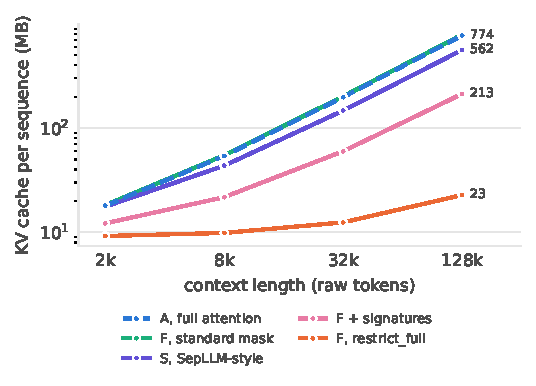
\includegraphics[width=0.55\textwidth]{figures/kv_vs_length.pdf}
\caption{Projected KV cache per sequence against context length. With the
standard mask, F overlaps the baseline A because the full-attention layers
keep every token. With \texttt{restrict\_full}, the cache grows with the
number of summaries (F), plus every kept signature (F + signatures) or
separator (S).}
\label{fig:kvlen}
\end{figure}

\section{Discussion}\label{sec:discussion}

\paragraph{Implications.}
Hybrid stacks that interleave local and global attention are now common.
In such models, summary tokens added only to the local layers compete with a
global path that sees every raw token. Under a short fine-tune, the model
takes the global path. Positive results for summary tokens in hybrid models
(e.g.\ \citealp{kwaisummary}) build the summaries into the architecture and
train on orders of magnitude more tokens. Our result suggests that the global-layer path, not the
placement of the summaries, decides whether they matter.

\paragraph{Closing the shortcut.}
We gave the full-attention layers the same mask as the sliding layers
(\texttt{restrict\_full}, $W=512$), so raw tokens more than $W$ back can
only be reached through \sumtok{}, and retrained F and G for 130 steps
(Table~\ref{tab:rf}). Far-raw attention in the full layers drops from 35\%
to zero, and long-range loss more than doubles (0.32 to 0.69--0.74 in both
seeds): distant code matters. The summaries do not recover it. Hiding them
still lowers long-range loss slightly in both seeds ($-0.008$ and $-0.014$
for F, $-0.004$ and $-0.001$ for G), so even as the only route past $W$ they
carry nothing the model uses at this training budget, and the hidden
condition, close to a StreamingLLM-style window with a sink
\citep{xiao2023sinks}, does as well. Fixed chunks (G) are at least as good as
scope parts (F) in both seeds (0.694 vs.\ 0.735 and 0.713 vs.\ 0.720), but
the margin depends on the seed.

\begin{table}[t]
\centering\small
\begin{tabular}{@{}lccccc@{}}
\toprule
& Heldout & Long-range & Long-range, & $\Delta$ & \sumtok{} attention \\
& loss & loss & \sumtok{} hidden & hide & sliding / full \\
\midrule
F, standard mask & 1.991 & 0.321 & -- & -- & -- \\
F, \texttt{restrict\_full} & 2.047 & 0.735 & 0.727 & $-0.008$ & 1.0\% / 0.6\% \\
G, \texttt{restrict\_full} & 2.048 & 0.694 & 0.690 & $-0.004$ & 1.5\% / 0.7\% \\
F, \texttt{restrict\_full} + signatures & 2.055 & 0.691 & 0.691 & $-0.0005$ & 0.6\% / 0.6\% \\
S (SepLLM-style), \texttt{restrict\_full} & 2.047 & 0.632 & -- & -- & -- \\
\bottomrule
\end{tabular}
\caption{Closing the global shortcut ($W=512$ in every layer). Long-range loss
more than doubles, and hiding the summaries still does not hurt. Keeping every
\texttt{def}/\texttt{class} line visible (last row) helps slightly, through the
signatures, not the summaries.}
\label{tab:rf}
\end{table}

\paragraph{Keeping signatures.}
A single \sumtok{} vector may hold what a function does, but code that calls
the function needs its exact name and parameters, and compressed tokens are
known to be poor at exact copying. We therefore add an option
(\texttt{keep\_signatures}) under which raw queries, in every layer when
combined with \texttt{restrict\_full}, also see every earlier \texttt{def}
or \texttt{class} line (including decorators), while function bodies stay
reachable only through \sumtok{}. Signature lines are 8.2\% of the raw
tokens in our training data, so every layer's cache grows by about 88
entries per 1{,}000 tokens (signatures plus summaries). Because the sliding
layers must now keep the signatures too, the projected cache at 128k tokens
is about 213~MB, 3.6$\times$ smaller than the full cache (774~MB) but larger
than with summaries alone (23~MB). We trained F with
\texttt{restrict\_full} and \texttt{keep\_signatures} for 130 steps. The
model does read the signatures (7.4\% of attention in the sliding layers,
8.7\% in the full layers), and long-range loss improves to 0.691 (0.694 with
seed 2; mean 0.693, against 0.728 for F and 0.704 for G). The gain is small
and consistent, remains more than twice the unrestricted 0.32, and comes with
a slightly worse all-token loss (0.777 vs.\ 0.761). Hiding the \sumtok{}s changes long-range loss by
$-0.0005$, so the small gain comes from the signatures, not the summaries.
Exact signatures are not what the lost distant context mainly provides.

\paragraph{A SepLLM-style baseline.}
Variant S has no \sumtok{} tokens: under \texttt{restrict\_full}, every layer
sees BOS, the last $W$ raw tokens and every earlier separator token
(whitespace and \texttt{.}~\texttt{,}~\texttt{?}~\texttt{!}~\texttt{;}~\texttt{:}),
the separator set of SepLLM \citep{chen2024sepllm}. It reaches a long-range
loss of 0.632 and 0.630 in two seeds, better than every \sumtok{} variant and the
signature variant. It is not memory-matched: separators are 24.0\% of the raw
tokens in our training data, against 8.2\% for signatures and 0.6\% for
summaries, so its projected cache at 128k tokens is 562~MB, against 213~MB
and 23~MB (774~MB for full attention). Figure~\ref{fig:tradeoff} shows the
resulting trade-off: keeping more raw tokens buys long-range accuracy, and at
this training budget a learned \sumtok{} buys none. Whether S still wins at
an equal memory budget is open.

\begin{figure}[t]
\centering
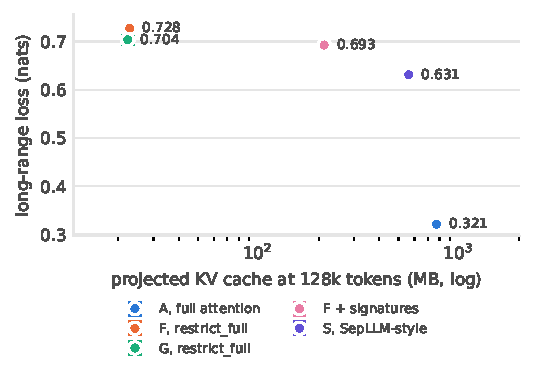
\includegraphics[width=0.55\textwidth]{figures/tradeoff.pdf}
\caption{Long-range loss against the projected KV cache at 128k tokens,
mean over two seeds (bars: range). Under
\texttt{restrict\_full}, quality improves only with the number of raw tokens
kept (signatures, separators); the summaries alone stay at the cheapest and
worst point.}
\label{fig:tradeoff}
\end{figure}

\paragraph{Threats to validity.}
\emph{Internal:} all variants share data, order, seed and hyper-parameters,
so differences come from the masks and segments; but with two seeds, gaps
below about 0.01 nats are not significant, and our conclusions rest only on
the larger, consistent effects (near-zero hiding effects across five settings,
and the doubling of long-range loss under \texttt{restrict\_full}).
\emph{Construct:} long-range loss scores identifier tokens defined more than
512 tokens earlier in another scope; it measures access to distant
definitions, not end-to-end code generation. \emph{External:} we study one
model (Gemma~4~E2B), one language (Python) and one corpus; models with
different attention layouts or much longer training may behave differently.

\paragraph{Limitations.}
The training is short: 3M tokens, rank-16 LoRA, two seeds per variant. The
probe and localization sets are small. The \sumtok{} embedding starts from a
reused token. Long-range loss uses one definition of long range (more than
512 tokens, across scopes). Longer training could teach the model to use the
summaries even with the global path open. Our results show only that it does
not do so at this budget, where the main effect of the method would be
expected to appear first.

\section{Conclusion}

Scope-aligned summary tokens retrofitted onto Gemma~4's sliding-window layers
do not improve language modelling, long-range identifier prediction or bug
localization over a no-summary baseline, even when the comparison is matched
for count and memory, and even when the local window is cut to 128 tokens.
The model ignores the summaries, because its full-attention layers already
reach distant code. Scope-aligned summary states are much more informative
than fixed-chunk ones, but only as informative as pooling the scope's own
tokens. Removing the global shortcut does not change this: with every layer
restricted to the last 512 tokens, distant code matters (long-range loss
more than doubles), but the summaries still carry nothing the model uses.
Keeping every function signature visible recovers only a small part of
the loss, and the summaries add nothing on top of it. A SepLLM-style
baseline that keeps every separator token does better than all of them, at
2.6 times the memory of the signature variant: at this budget, long-range
quality follows how many raw tokens are kept, not learned summaries. Making
summary tokens useful for code would likely need much longer training than
our 3M tokens.

\begin{thebibliography}{99}
\bibitem[Mu et al.(2023)]{mu2023gist}
J.~Mu, X.~L. Li, and N.~Goodman. Learning to compress prompts with gist tokens.
\emph{NeurIPS}, 2023. arXiv:2304.08467.
\bibitem[Chevalier et al.(2023)]{chevalier2023autocompressor}
A.~Chevalier, A.~Wettig, A.~Ajith, and D.~Chen. Adapting language models to
compress contexts. \emph{EMNLP}, 2023. arXiv:2305.14788.
\bibitem[Ge et al.(2024)]{ge2023icae}
T.~Ge, J.~Hu, L.~Wang, X.~Wang, S.-Q. Chen, and F.~Wei. In-context autoencoder
for context compression in a large language model. \emph{ICLR}, 2024.
arXiv:2307.06945.
\bibitem[Zhang et al.(2024)]{zhang2024beacon}
P.~Zhang et al. Long context compression with activation beacon.
arXiv:2401.03462, 2024.
\bibitem[Chen et al.(2024)]{chen2024sepllm}
G.~Chen et al. SepLLM: Accelerate large language models by compressing one
segment into one separator. arXiv:2412.12094, 2024.
\bibitem[Xiao et al.(2024)]{xiao2023sinks}
G.~Xiao, Y.~Tian, B.~Chen, S.~Han, and M.~Lewis. Efficient streaming language
models with attention sinks. \emph{ICLR}, 2024. arXiv:2309.17453.
\bibitem[Hu et al.(2022)]{hu2021lora}
E.~J. Hu et al. LoRA: Low-rank adaptation of large language models.
\emph{ICLR}, 2022. arXiv:2106.09685.
\bibitem[Kocetkov et al.(2022)]{kocetkov2022stack}
D.~Kocetkov et al. The Stack: 3 TB of permissively licensed source code.
arXiv:2211.15533, 2022.
\bibitem[Jimenez et al.(2024)]{jimenez2023swebench}
C.~E. Jimenez et al. SWE-bench: Can language models resolve real-world GitHub
issues? \emph{ICLR}, 2024. arXiv:2310.06770.
\bibitem[Tarasov et al.(2025)]{sentgist}
D.~Tarasov, E.~Goncharova, and A.~Kuznetsov. Sentence-anchored gist
compression for long-context LLMs. arXiv:2511.08128, 2025.
\bibitem[Chu et al.(2026)]{kwaisummary}
C.~Chu, G.~Zhou, G.~Zhang, H.~Li, H.~Peng, et al. Kwai Summary Attention
technical report. arXiv:2604.24432, 2026.
\bibitem[Chen et al.(2026)]{codecomp}
Q.~Chen, J.~Xiong, C.~Zhao, S.~Yang, and N.~Wong. CodeComp: Structural KV
cache compression for agentic coding. arXiv:2604.10235, 2026.
\bibitem[Mao et al.(2026)]{hssa}
Y.~Mao, M.~Y. Li, and E.~B. Fox. Simplified sparse attention via gist tokens.
arXiv:2604.20920, 2026.
\bibitem[Li et al.(2025)]{admtree}
Y.~Li, S.~Chen, Y.~Li, Y.~Chen, H.-T. Zheng, H.~Wang, W.~Jiang, and P.~S. Yu.
AdmTree: Compressing lengthy context with adaptive semantic trees.
arXiv:2512.04550, 2025.
\bibitem[Yang et al.(2026)]{skipcompressor}
X.~Yang, R.~Chatterjee, H.~Udupi, V.~Ramavarapu, and C.~Zhai. Skip the
compressor: Coding agents fix more issues when they pick whole files.
arXiv:2610.21073, 2026.
\end{thebibliography}

\end{document}
